\silentlychangedin{1C}{1C-figures}{

\begin{onecolumnfigure}[!ht]
\includegraphics[width=0.7\linewidth]{figures/figure-map-location.pdf}
\end{onecolumnfigure}

}{

\begin{onecolumnfigure}[t]

\begin{fitheight}{3.2\standardhexwidth}
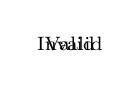
\begin{tikzpicture}
    \setfiguresize{-2.5}{-1.6}{+2.5}{+1.6}
    \drawevenhexgrid{-2}{-1}{5}{3}
    \drawaircraftcounter{-1.00}{+0.50}{90}{F-4}{}{}
    \drawaircraftcounter{-1.50}{-0.75}{120}{F-4}{}{}
    \drawaircraftcounter{+1.00}{+0.00}{90}{F-4}{}{}
    \miniathex{-2.00}{+0.00}{\node {\scriptsize Valid};}
    \miniathex{+2.00}{+0.00}{\node {\scriptsize Invalid};}
\end{tikzpicture}
\end{fitheight}


\figurecaption{figure:aircraft-map-location}{\protect\x{Map Location.}{Aircraft and missiles may be located either in hexes or on hex sides. When located in a hex, it must face towards one of the sides or one of the corners. When located on a hex side, it must face along the hex side. The two aircraft on the left have valid locations and facings. The aircraft on the right has a valid location but invalid facing.}}

\end{onecolumnfigure}

}


